\chapter{A granular credit register}\label{ch:credit}

Ask a disclosure control officer what a minimum cell count costs, and the answer
usually comes as a count of records. A floor of ten removes 4 per cent of the loans;
a floor of twenty removes 15 per cent.
% source: artifacts-robustness/robustness.json (coverage: loan_share 0.958 at k=10, 0.851 at k=20)
The answer is honest and it is the one release documents print, because records are
what the rule acts on and what the software counts. Behind it sits a belief that
most practitioners hold without stating it: suppression costs data in proportion to
the records it removes. On that belief a file that keeps four loans in five has kept
four fifths of what its users wanted, and a committee can weigh protection against
loss by reading one percentage.

The belief is reasonable for a file whose records are roughly alike in the analyses
they feed. A credit register is not such a file. On the synthetic register of this
chapter, the floor that a history-aware adversary requires keeps 20 per cent of the
loans and 4 per cent of the exposure, and it keeps no loan to a large firm.
% source: paper/generated/table_robustness.tex (floor 150: loans 20%, exposure 4%); bis_ifc_full.tex l.2240-2243 (no loan to a large firm)
The records that a floor removes first are the ones in thin cells, and in a credit
register the thin cells hold the largest borrowers, whose loans carry most of the
money. Counting records measures the wrong loss.

\begin{mdframed}[linecolor=black,linewidth=0.8pt,backgroundcolor=gray!8,innerleftmargin=8pt,innerrightmargin=8pt]
\textbf{Read this before the floors.} The floors of 75, 150 and ``none'' in this chapter, and
in every chapter that quotes them, are properties of a synthetic register under declared
parameters. The generator's parameters were chosen, not estimated from a real register. The
adversary's reading precision, 0.6 on the log scale, was not measured. The panel has no
originations or exits in the frozen case and a simplified dynamic model in the changing
case. The key of sector, region and size class may match no real register. These floors are
not recommendations for any real register. The decision rule that produced them is the
transferable result. Section~\ref{app:b-precision} shows how an institution argues for its
own precision.
\end{mdframed}

This chapter asks one question: \emph{for each adversary an institution might
declare against a loan-level release of its credit register, what minimum cell count
does a tolerance require, and what is left of the file once that floor is applied?}
The answer runs through the register itself, the five harms it can cause, an
adversarial evaluation of five protection policies, the floors that fixed-sequence
testing selects for six adversaries, what those floors keep, and how far the floors
move when the tolerance, the register draw and the adversary's precision change.

\section{Why the register is synthetic}

\begin{practicebox}{The numbers here belong to the example}
Every floor, tolerance and reading precision in this chapter was chosen or generated for the synthetic register. None is a standard, and none transfers to a real programme. Take the procedure from this chapter and not the numbers.
\end{practicebox}


Chapter~\ref{ch:decision} introduced the register briefly. It is built to share the
structure of a supervisory loan-level collection. In the euro area, AnaCredit
collects, mostly monthly, data on loans by credit institutions to legal entities
whenever the debtor's commitment with the reporting institution is at least
EUR~25{,}000, and each record ties a borrower to a lender
\citep{ecb2016,israel2017}.
% source: paper/bis_ifc_full.tex l.1845-1850
Registers of this kind support research on credit supply that could not be done any
other way: \citet{khwaja2008} use a credit register to separate supply from demand,
and \citet{jimenez2012} use loan applications in the Spanish register to identify
the bank balance-sheet channel. Loan-level data of this kind are not released for
general use, and research access is restricted. That is why the register here is
synthetic, and it is also why its parameters are chosen and not estimated: there is
no released file from which to estimate them.

The generator draws 20{,}000 borrowers, each with a sector from 18, a region from
12 and a size class from four, so the borrower key has $18 \times 12 \times 4 = 864$
cells. Size classes are drawn with probabilities 0.62, 0.24, 0.11 and 0.03, so large
firms are three borrowers in a hundred. Each borrower has between one and four
lending relationships, drawn as one plus a binomial count on three trials whose
success probability rises from 0.10 for the smallest firms to 0.70 for the largest,
so most small firms have one lender and most large firms have several. Lenders are
chosen from 60 with skewed shares; the largest holds 23 per cent of relationships.
Exposure is lognormal within size class, with log means 11, 12.5, 14 and 16 and a
log standard deviation of 0.8, so a typical large-firm loan is about 150 times a
typical micro-firm loan. Arrears are drawn at a rate between 3 and 10 per cent that
varies with sector and size, about 7 per cent overall.
% source: src/privacy_risk/credit.py, make_credit_register (size probabilities, relationships, log means, sd 0.8, arrears rate); configs/paper.json (20,000 borrowers, 60 lenders, 18 sectors, 12 regions, 4 size classes, 6 months); paper/bis_ifc_full.tex l.1871-1882 (864 cells, 7 per cent arrears, largest lender 23 per cent)

Six monthly vintages are generated as a panel with a stable stock. Most loans are
outstanding when the panel opens; the others are originated in a month drawn
uniformly from the second to the sixth. Every loan then leaves with a monthly hazard
of 0.04 and does not return. Over the six months 32{,}581 loans are observed, the
first release holds 27{,}167 of them, the stock stays near 27{,}000, and 81 per cent
of the loans in the first release are live in all six vintages.
% source: paper/bis_ifc_full.tex l.1874-1880; src/privacy_risk/credit.py (exit_hazard 0.04)
The difference, 5{,}414 loans, is the sixth of the observed loans that were
originated during the panel.

Each choice was made to reproduce a structural feature that bears on disclosure: a
skewed lender market, several relationships per large borrower, a thin top size
class, and monthly entry and exit. None was fitted to data. Two simplifications bear
directly on the results and must be kept in view. A loan's exposure is the same in
every vintage in which it is live, where a real register reports outstanding amounts
that change as loans are drawn and repaid. And whether a loan is live in a month is
drawn independently of its key and exposure, where in a real register large loans
may run longer. Every floor in this chapter is a floor for this design. It describes
a class of release systems with these features, and the way to refute it is to run
the same evaluation inside an institution that holds the real file.

Tomás arrives at the Bank with a research proposal on credit to large firms. He
asks for the loan-level file for six months: each loan with its sector, region,
size class and exposure, under a pseudonym that lets him follow a loan from month to
month. Naledi reads the request twice. The fields are the ones the register was
built around, and his research question is about the borrowers in its thinnest
cells.

\section{Five harms from one register}\label{c13:sec-harms}

A single risk figure covers one harm, and a credit register can cause five. A
borrower may be identified. A borrower--lender relationship may be alleged, whether
or not the borrower is identified. Arrears status may be inferred for a class of
borrowers without identifying anyone. One lender's contribution may be reconstructed
from published totals by another participant. And two consecutive vintages may be
differenced. Table~\ref{c13:tab-harms} reports all five against one lever, a minimum
cell count $k_{\min}$ on the borrower key, applied to the first release.

\begin{table}[ht]
\centering
\caption{Five harms and one utility on the synthetic credit register under a minimum
cell count on the borrower key. Identification is the share of released
relationships the attack recovers, with its exact one-sided 95 per cent bound, and
again for the largest size class. The predictive value is that of an alleged
borrower--lender relationship. Status disclosed is the share of large borrowers whose
key class is homogeneous in arrears status. Utility is the negative weighted loss
over the four analyses the register is collected for.}
\label{c13:tab-harms}
\small\setlength{\tabcolsep}{4pt}
\begin{tabular}{rrrrrrrr}
\toprule
$k_{\min}$ & Kept & Ident. & Bound & Large firms & Relationship PPV & Status & Utility \\
\midrule
1  & 1.000 & 0.0855 & 0.0931 & 0.247 & 0.328 & 0.444 & $-0.000$ \\
5  & 0.990 & 0.0770 & 0.0843 & 0.273 & 0.324 & 0.381 & $-0.050$ \\
10 & 0.958 & 0.0705 & 0.0775 & 0.119 & 0.320 & 0.262 & $-0.139$ \\
20 & 0.851 & 0.0563 & 0.0626 & 0.155 & 0.313 & 0.119 & $-0.254$ \\
\bottomrule
\end{tabular}
% source: paper/generated/table_credit.tex
\end{table}

\paragraph{Identification is a subgroup problem.} The attack recovers the exact
relationship for 0.0855 of released rows, with a bound of 0.0931. Recovering the right
borrower succeeds for 0.1095, because a borrower with several lenders can be found
through any of them.
% source: paper/generated/table_credit.tex; paper/bis_ifc_full.tex l.1891-1895 (0.1095)
Both look comfortable as averages. Split by size class, the relationship figure is
0.050, 0.091, 0.128 and 0.247, so a large borrower faces about five times the risk
of a micro borrower.
% source: paper/bis_ifc_full.tex l.1896-1898
The large-firm column of Table~\ref{c13:tab-harms} is not monotone in the floor: it
is 0.273 at $k_{\min}=5$ and 0.119 at $k_{\min}=10$; read the whole column as noisy. The class rests on few targets
in a uniform draw, and its interval at $k_{\min}=1$, $[0.192, 0.309]$, overlaps the
interval at $k_{\min}=20$, $[0.085, 0.250]$.
% source: paper/generated/numbers.tex (runcreditidentificationlargelow/high, ...strictlow/high)
The large-firm figure at no suppression agrees across independent draws: 0.248 in
the policy comparison below, and about 0.24 on a stratified draw of 4{,}000
large-firm targets. This is why the subgroup floors later in the chapter use a
stratified draw.
% source: paper/bis_ifc_full.tex l.1904-1910

\paragraph{An alleged relationship is a base-rate statement.} Suppose the adversary
names, for every released borrower, the lender holding the largest share of that
borrower's key class. What counts for harm is the probability that an allegation is
true, which Bayes' theorem gives from the prevalence $p$ of a borrower--lender pair,
the sensitivity $s$ of the rule and its specificity $q$:
\begin{equation}\label{c13:eq-ppv}
\Prob(\text{true} \mid \text{alleged}) = \frac{ps}{ps + (1-p)(1-q)} .
\end{equation}
On the register $p = 0.0243$, $s = 0.225$ and $q = 0.9885$, which is 0.989 to three
places, and \eqref{c13:eq-ppv} returns 0.328, the realised share of correct allegations.
The rounded 0.989 would return 0.337, so the unrounded specificity is the one to carry.
% source: paper/bis_ifc_full.tex l.1914-1920; paper/generated/numbers.tex (runcreditppv 0.328)
A specificity of 0.989 sounds protective and is not, because the prevalence is low.
An allegation right a third of the time is 1.4 times the success rate of always
naming the largest lender in the market, whose share is 0.23, and it is wrong about
two borrowers in three. The floor barely moves it: 0.328 at $k_{\min}=1$ and 0.313
at $k_{\min}=20$.
% source: paper/generated/numbers.tex (runcreditppvlift 1.4, runcreditppvstrict 0.313)
The lever that governs identification does not govern relationship disclosure.

\begin{example}[Ten thousand pairs]\label{c13:ex-pairs}
Count instead of multiplying. Among 10,000 possible borrower--lender pairs, 243 are real
($p = 0.0243$). The rule names the right lender for 22.5 per cent of them, about 54.7
pairs. Of the 9,757 pairs that are not real, it wrongly names 1.15 per cent ($1 - q$),
about 112.2 pairs. So the rule makes about 166.9 allegations, of which 54.7 are true:
$54.7/166.9 = 0.328$. Two allegations in three are false although the rule is wrong about
only one false pair in 87, because false pairs outnumber real ones forty to one. Naledi
used this count when the chair asked why a specificity of 0.99 was not reassuring.
\end{example}


\paragraph{Status can be disclosed without identification.} A key class whose members
all share an arrears status discloses that status for every member, whatever the
size of the class. For large borrowers 44.4 per cent of released relationships sit in
such a class at $k_{\min}=1$, falling to 11.9 per cent at $k_{\min}=20$.
% source: paper/generated/numbers.tex (runcreditstatuslarge 0.444, runcreditstatuslargestrict 0.119)
In this register every homogeneous class is homogeneous in the benign direction,
because arrears are rare, so what is disclosed is the absence of arrears. That is a
property of the chosen base rate. On a real register a small sector--region cell in
distress is the case to look for, and the attribute criteria of
\citet{machanavajjhala2007} and \citet{li2007} address it by changing the risk model,
which a cell count does not.

\paragraph{Published totals give contributions away by subtraction.} Totals by
region, sector and size class form a linear system. In the first vintage 2.0 per cent
of the 814 published cells have a single contributor, so that lender's position is
the published total, and 3.9 per cent have two, so either participant recovers the
other's amount by subtraction. Together they hold 2.8 per cent of total exposure.
Requiring five contributors in place of three suppresses 14.4 per cent of cells in
place of 5.9 per cent.
% source: paper/bis_ifc_full.tex l.1955-1962
With lender shares up to 23 per cent, one contributor can estimate another's amount
closely even when three or more contribute, which is what the dominance and $p\%$
rules for magnitude tables are designed to catch \citep[ch.~4]{hundepool2012}. They
are not evaluated here. The loan-level floor leaves this risk untouched.

\paragraph{Monthly vintages can be differenced.} When a published count moves by
one between vintages, the change in the published total is the arriving or departing
amount, provided one loan moved. The adversary does not see how many loans moved,
and Proposition~\ref{c13:prop-diff} gives the posterior that a unit change was a
single move.

\begin{proposition}[Differencing posterior]\label{c13:prop-diff}
Let the arrivals $A$ and departures $D$ of a published cell between two vintages be
independent Poisson variables with common mean $\lambda > 0$. Then
\begin{equation}\label{c13:eq-diff}
\Prob\bigl(A + D = 1 \bigm| |A - D| = 1\bigr)
= \Bigl(\sum_{d=0}^{\infty} \frac{\lambda^{2d}}{d!\,(d+1)!}\Bigr)^{-1}
= \frac{\lambda}{I_1(2\lambda)},
\end{equation}
where $I_1$ is the modified Bessel function of the first kind. The posterior is
strictly decreasing in $\lambda$ and tends to one as $\lambda \to 0$.
\end{proposition}

The proposition turns an intuition into a number: a unit change in a quiet cell
almost certainly reveals one loan, and in a busy cell it may be offsetting moves.
\begin{example}[A quiet cell and a busy one]\label{c13:ex-cells}
The rates are illustrative. In a cell of large firms in a small region, a loan arrives
or leaves about once in ten months, so $\lambda = 0.1$. Equation~\eqref{c13:eq-diff}
gives $0.1/I_1(0.2) = 0.995$: when the published count moves by one, the change in the
published total is one loan's exposure with near certainty. In a cell of micro firms with
$\lambda = 1.35$, the pooled rate on the register, the posterior is 0.448, and a unit
change is more likely than not to hide offsetting moves. At $\lambda = 3$ it is 0.049.
Naledi's monthly series carries both kinds of cell, and the quiet ones are those of the
large borrowers Tom\'as wants to study.
\end{example}

Across consecutive months 36.1 per cent of comparable cell pairs show a unit change

at a count floor $c_{\min}=1$, and 39.0 per cent at $c_{\min}=10$, because a higher
count floor keeps only the busier cells, where counts move more.
% source: paper/bis_ifc_full.tex l.1975-1979
Which rate enters \eqref{c13:eq-diff} decides the answer. Pooled over all cells,
arrivals and departures together average 2.7 per cell per transition, so
$\lambda = 1.35$ and the posterior is 0.45. Evaluated at the rate of each cell that
shows a unit change and averaged, it is 0.65, and the realised share of unit changes
that were in fact a single move is also 0.65.
% source: paper/bis_ifc_full.tex l.1981-1988; src/privacy_risk/credit.py differencing_risk (posterior_single_move_per_cell averages the per-cell posterior)
The pooled rate understates the exposure, and the institution, which holds the
register, can count realised single moves directly. At $c_{\min}=10$ a unit change
still reveals one loan's exposure in 56 per cent of cases.
% source: paper/bis_ifc_full.tex l.1990-1991

Naledi takes Table~\ref{c13:tab-harms} to the chair before any floor is chosen. The
table has one row per floor and five columns of harm, and only the first column
moves much. ``Which of these is Tomás's file?'' the chair asks. The honest answer is
the identification column, because his file is the loan-level one; the other four
belong to the aggregates and the monthly series the Bank already publishes.

\section{An adversarial evaluation}\label{c13:sec-eval}

The rest of the chapter fixes an adversary and a set of attacks and runs them
against five protection policies on the same register, with one body of auxiliary
information. The reporting follows the practice for attacks on trained models: how
often an attack succeeds, how often it is right when it acts, and what it must know
before it can act at all \citep{shokri2017,carlini2022}.

\subsection{The adversary and the attack}

The adversary targets one borrower. It holds the sector, region and size class
exactly, which is the natural case for a credit register, where these are
public facts. It holds a reading of the loan's log exposure with Gaussian error of
standard deviation 0.6, either once or once for every vintage in which the loan is
live. In some attacks it also knows the loan's history, the set of vintages in which
the loan is live.
% source: paper/bis_ifc_full.tex l.2034-2041; configs/paper.json (covariate_sd 0.6)

The history needs an argument, because it is what lets pooling help. The borrower
knows its own loan, and so do the lender and any counterparty to it, such as a
guarantor or a buyer of the loan. Public records can reveal it too, where a register
of charges over company assets is public or a firm reports its borrowing in a filing.
A journalist or researcher who knows a firm's sector, region and size will not in
general know in which months a particular loan was drawn or repaid. The evaluation
therefore reports every pooled attack with and without the history, and the
institution declares which adversary it guards against.

The attack blocks on region, keeps the loans in the first release whose key agrees
with the target's, scores each candidate by the log density of the exposure readings
under the adversary's error model, and names the highest-scoring candidate. The
pooled attack uses every vintage. With the history, it excludes every candidate whose
pattern of appearances differs from the target's in any vintage, through a penalty of
30 on the log score for each mismatch; since the target always matches, a mismatched
candidate is in effect removed. With one reading per vintage, the extra readings
amount to one more precise reading of the same exposure.
% source: paper/bis_ifc_full.tex l.2060-2075
Figure~\ref{c13:fig-history} shows the history test on four loans in one cell.

\begin{figure}[ht]
\centering
\begin{tikzpicture}[x=1.0cm,y=0.62cm,font=\small]
  \tikzset{live/.style={draw,fill=gray!55,minimum width=0.8cm,minimum height=0.42cm},
           gone/.style={draw,pattern=north east lines,pattern color=gray!70,minimum width=0.8cm,minimum height=0.42cm}}
  \foreach \m in {1,...,6} {\node at (\m,1) {$v=\m$};}
  \node[anchor=east] at (0.4,0) {target $t$};
  \foreach \m/\s in {1/live,2/live,3/live,4/live,5/gone,6/gone} {\node[\s] at (\m,0) {};}
  \node[anchor=east] at (0.4,-1.2) {candidate $a$};
  \foreach \m/\s in {1/live,2/live,3/live,4/live,5/gone,6/gone} {\node[\s] at (\m,-1.2) {};}
  \node[anchor=east] at (0.4,-2.2) {candidate $b$};
  \foreach \m/\s in {1/live,2/live,3/live,4/live,5/live,6/live} {\node[\s] at (\m,-2.2) {};}
  \node[anchor=east] at (0.4,-3.2) {candidate $c$};
  \foreach \m/\s in {1/live,2/live,3/gone,4/gone,5/gone,6/gone} {\node[\s] at (\m,-3.2) {};}
  \node[anchor=west] at (6.7,-1.2) {kept: same pattern};
  \node[anchor=west] at (6.7,-2.2) {excluded: live where $t$ is absent};
  \node[anchor=west] at (6.7,-3.2) {excluded: absent where $t$ is live};
  \draw[dashed] (0.5,-0.6) -- (11.6,-0.6);
  \node[live,minimum width=0.5cm] at (1.2,-4.5) {};
  \node[anchor=west] at (1.5,-4.5) {published in that vintage};
  \node[gone,minimum width=0.5cm] at (6.2,-4.5) {};
  \node[anchor=west] at (6.5,-4.5) {not published};
\end{tikzpicture}
\caption{How the pooled adversary uses a loan's history. All four loans share the
target's key cell. An adversary who knows the vintages in which the target is live
keeps only candidates whose pattern matches the target's in every vintage, and then
ranks the survivors by its exposure readings. Shade and hatching both mark the two
states.}
\label{c13:fig-history}
\end{figure}

Without the history the other vintages add nothing. Proposition~\ref{prop:nohistory}
of Chapter~\ref{ch:programmes} proves this under the two simplifications of the
generator: published values repeat across vintages, and whether a loan is live is
independent of them. The gain from pooling on this register therefore lives in the
history, and on a register whose published fields change from month to month the
proposition would not apply.

\subsection{Five policies}

Five loan-level policies enter the comparison. They are stylised versions of rules
described by \citet{hundepool2012}, not copies of any institution's practice: no
suppression; a threshold rule that withholds a cell unless at least three lenders
contribute; the same rule with a heuristic secondary suppression that also withholds
the smallest surviving cell in each region; and $k$-anonymity on the borrower key at
$k=5$ and $k=10$. The secondary suppression is not audited against the sector and
size margins, so it is not secondary suppression in the sense of \citet{cox1980} and
\citet{fischetti2001}. Table~\ref{c13:tab-eval} gives the outcomes, each from 4{,}000
attacks on independently drawn targets.
% source: paper/bis_ifc_full.tex l.2101-2102, 2115-2136

\begin{table}[ht]
\centering
\caption{Attack outcomes by policy on the synthetic register, tolerance 0.12. Release
and pooled give the share of targets named correctly for one release and over six
vintages (pooled attack with a reading per vintage and the history). Precision is
over the attempts whose posterior passes one half, and acts is how often that
happens. The last two columns give the size class with the highest rate and its
exact 95 per cent upper bound.}
\label{c13:tab-eval}
\small\setlength{\tabcolsep}{4pt}
\begin{tabular}{lrrrrrrrr}
\toprule
Policy & Kept & Utility & Release & Pooled & Precision & Acts & Worst class & Bound \\
\midrule
No suppression            & 27{,}167 & $-0.000$ & 0.089 & 0.260 & 0.716 & 0.020 & 0.248 & 0.297 \\
Three contributors        & 27{,}068 & $-0.019$ & 0.084 & 0.255 & 0.822 & 0.018 & 0.180 & 0.228 \\
Secondary suppression     & 27{,}027 & $-0.028$ & 0.080 & 0.259 & 0.746 & 0.015 & 0.156 & 0.203 \\
$k$-anonymity, $k=5$      & 26{,}885 & $-0.050$ & 0.074 & 0.269 & 0.771 & 0.012 & 0.183 & 0.234 \\
$k$-anonymity, $k=10$     & 26{,}019 & $-0.139$ & 0.070 & 0.244 & 0.800 & 0.009 & 0.141 & 0.193 \\
\bottomrule
\end{tabular}
% source: paper/generated/table_evaluation.tex
\end{table}

Four results come out of Table~\ref{c13:tab-eval}. Every suppression policy reduces
the per-release risk and none removes it: from 0.089 with no suppression to 0.070
under $k=10$. The reduction is modest because the exposure reading separates
candidates inside a cell however large the cell is, and every policy meets the
tolerance of 0.12 on one release.

The same policies do far less against the pooled attack, which lies between 0.244
and 0.269 for all five. Under $k=5$ the per-release 0.074 becomes 0.269, the largest
gap in the table at 0.195.
% source: paper/generated/table_evaluation.tex; paper/generated/numbers.tex (runevallargestgap 0.195)
Table~\ref{c13:tab-decomp} separates the two sources of the gap on the same targets.
Under no suppression, six readings against one release raise the rate from 0.089 to
0.158; pooling six vintages with one reading raises it to 0.191, with a bound of
0.201, already above the tolerance; with both the rate is 0.260. On this register
the two effects add with almost no interaction, and for the adversary with the
history the programme finding does not rest on the extra readings.

\begin{table}[ht]
\centering
\caption{Where the pooled excess comes from: share of targets named correctly, with
the exact 95 per cent upper bound in brackets, changing one factor at a time on the
same targets. All pooled attacks know the history.}
\label{c13:tab-decomp}
\small\setlength{\tabcolsep}{4pt}
\begin{tabular}{lrrrr}
\toprule
 & \multicolumn{2}{c}{One release} & \multicolumn{2}{c}{Six vintages} \\
\cmidrule(lr){2-3}\cmidrule(lr){4-5}
Policy & one reading & six readings & one reading & six readings \\
\midrule
No suppression       & 0.089 (0.097) & 0.158 (0.168) & 0.191 (0.201) & 0.260 (0.272) \\
$k$-anonymity, $k=5$ & 0.074 (0.081) & 0.141 (0.150) & 0.183 (0.194) & 0.269 (0.281) \\
$k$-anonymity, $k=10$& 0.070 (0.076) & 0.130 (0.139) & 0.179 (0.190) & 0.244 (0.256) \\
\bottomrule
\end{tabular}
% source: paper/generated/table_decomposition.tex
\end{table}

The adversary is often right when it acts, and it seldom acts on one release. Under
$k=5$ it passes the decision threshold on 48 of 4{,}000 attempts and is right on 37 of
those, a precision of 0.771 resting on 48 decisions, or about 108 attempts per
correct identification.
% source: paper/bis_ifc_full.tex l.2177-2182
An evaluation that reports only the average hides the precision, and one that reports
only the precision hides how few attempts it rests on.

The average also conceals a subgroup. With no suppression the largest-firm class
reaches 0.248, with a bound of 0.297, and no row of Table~\ref{c13:tab-eval} passes a
subgroup control at 0.12 even on one release.
% source: paper/generated/table_evaluation.tex
Large borrowers are few, so their cells are small and their exposures far apart, and
both effects push the same way. The three other attacks are indifferent to the lever:
under $k=5$ an alleged relationship is true 0.324 of the time, a unit change is a
single move 0.623 of the time, and a confident reading of arrears status is right
0.946 of the time against 0.929 for guessing no arrears for everyone, a gain of 0.017.
% source: paper/bis_ifc_full.tex l.2198-2203

Naledi's assessment of Tomás's file, one release at a time, passes with no
suppression. She writes the result into a draft record and then adds a line she has
learned to add: the file goes out monthly, and the pseudonym persists. The release
she assessed is not the release Tomás will hold.

\section{The floor each adversary requires}\label{c13:sec-floors}

Fix the tolerance at $\tau=0.12$ and choose the minimum cell count by the exact upper
bound. Because the level is chosen from a grid by the same bounds that certify it,
the choice uses fixed-sequence testing (Chapter~\ref{ch:selection}): levels are
tested from $k_{\min}=300$ down on one draw of 4{,}000 targets, the procedure stops
at the first level whose bound exceeds the tolerance, and the floor is the last level
that passed. The chosen level is then audited on a second, independent draw. Where
confirmation fails, the next stricter level is confirmed on the same fresh draw.
% source: paper/bis_ifc_full.tex l.2210-2222

The adversary who pools six vintages with one reading and knows the history shows
how the procedure runs. On the selection draw the upper bounds, from the strictest
level down, are 0.042 at 300, 0.059 at 200, 0.073 at 150, 0.081 at 100, 0.101 at 75,
0.111 at 50 and 0.139 at 40. The sequence stops at 40 and selects 50. On the fresh
draw, 50 gives 458 successes in 4{,}000, a rate of 0.1145 with a bound of 0.1231, and
fails. The next stricter level, 75, gives 384 in 4{,}000, a rate of 0.096 with a bound
of 0.104, and is confirmed.
% source: artifacts-robustness/worked_examples.json (example_selection: selection_upper, confirm_50, confirm_75)
The selection step carries the error bound; the confirmation guards against
reporting a floor that passed by chance near the tolerance, which is what happened
at 50. Table~\ref{c13:tab-floors} gives the result for six adversaries.

\begin{table}[ht]
\centering
\caption{The floor each adversary requires on the synthetic register, tolerance 0.12.
Floors are chosen by fixed-sequence testing from $k_{\min}=300$ down on 4{,}000
targets and confirmed on a second draw (rate, with exact 95 per cent upper bound).
Loans and exposure are the percentages of the first release kept. The subgroup floor
requires every size class to meet the tolerance, with the largest firms on a
stratified draw, from $k_{\min}=200$ down; it was not confirmed on a second draw.
``None'' means no level up to the top of the grid passes.}
\label{c13:tab-floors}
\small\setlength{\tabcolsep}{3pt}
\begin{tabular}{lrrrrr}
\toprule
Adversary & Floor & Confirmation & Loans & Exposure & Subgroup \\
\midrule
One release, one reading                      & 1    & 0.084 (0.092) & 100 & 100 & 20 \\
Six vintages, one reading, no history         & 1    & 0.083 (0.091) & 100 & 100 & -- \\
Six vintages, one reading, history            & 75   & 0.096 (0.104) & 45  & 11  & 200 \\
Six vintages, reading per vintage, no history & 20   & 0.105 (0.114) & 85  & 52  & -- \\
Six vintages, reading per vintage, history    & 150  & 0.101 (0.109) & 20  & 4   & none \\
Insider: exact exposure, history              & none & --            & --  & --  & -- \\
\midrule
\multicolumn{6}{l}{\emph{Exposure published to one significant figure}}\\
One release, one reading                      & 1    & 0.079 (0.086) & 100 & 100 & -- \\
Six vintages, one reading, history            & 50   & 0.111 (0.119) & 58  & 20  & -- \\
Six vintages, reading per vintage, history    & 150  & 0.085 (0.092) & 20  & 4   & -- \\
Insider: exact exposure, history              & none & --            & --  & --  & -- \\
\bottomrule
\end{tabular}
% source: paper/generated/table_robustness.tex
\end{table}

Read down the first block and the floor climbs with what the adversary knows. Against
one release the floor is 1, no suppression, with a confirmation rate of 0.084 and a
bound of 0.092. Pooling six vintages without the history adds nothing, as
Proposition~\ref{prop:nohistory} predicts: the floor stays at 1 and the confirmation
is 0.083 (0.091). With the history the floor is 75. With a reading per vintage and no
history it is 20, and with both it is 150, confirmed at 0.101 (0.109). The insider,
who knows the history and reads exposure with a standard deviation of 0.01 on the log
scale, is not stopped by any floor: its success is 0.772 at $k_{\min}=1$ and still
0.416 at $k_{\min}=300$.
% source: paper/generated/table_robustness.tex; paper/bis_ifc_full.tex l.2253-2256 (0.772, 0.416); artifacts-robustness/robustness.json (insider_sd 0.01)

The insider's result is not an accident of the grid. A precise reading separates
candidates in a cell of any size, and Proposition~\ref{c13:prop-insider} says by how
much.

\begin{proposition}[A precise reading defeats any floor]\label{c13:prop-insider}
Let the candidates for a target $t$ have published log exposures $x_1,\dots,x_n$, let
the adversary read $y = x_t + e$ with $e \sim N(0,\sigma^2)$, and let it name a
candidate that maximises the Gaussian likelihood, breaking ties uniformly at random.
\begin{enumerate}
\item If the gap $g = \min_{j \ne t} |x_j - x_t|$ is positive, the attack names the
target with probability at least $2\Phi\bigl(g/(2\sigma)\bigr) - 1$, whatever the number $n$ of
candidates; for fixed published values this tends to one as $\sigma \to 0$.
\item If $r - 1 \ge 1$ other candidates publish the same value as the target, the
attack names the target with probability at most $1/r$, whatever $\sigma$.
\end{enumerate}
\end{proposition}

The first part is why a floor cannot stop the insider: a floor bounds $n$ from below,
and the bound in part 1 does not depend on $n$. A larger cell does shrink the typical
gap $g$, which is why the insider's success falls from 0.772 to 0.416 across the grid
without approaching the tolerance. The second part is why rounding works on the
insider where floors do not. Published to one significant figure, exposures tie, and
the insider's success at $k_{\min}=1$ halves, to 0.388. The outside adversaries,
whose readings are already coarse, barely notice the rounding: their floors are 1,
50 and 150.
% source: paper/bis_ifc_full.tex l.2297-2302; paper/generated/table_robustness.tex

\begin{example}[Pieter's reading of one loan]\label{c13:ex-pieter}
The inputs are illustrative. A cell holds four loans with log exposures 11.6, 12.0, 12.1
and 12.9, and the target is the loan at 12.0. The nearest other loan is 0.1 away, so
$g = 0.1$. For an outside adversary with $\sigma = 0.6$, part 1 of
Proposition~\ref{c13:prop-insider} guarantees only $2\Phi(0.1/1.2) - 1 = 0.066$; its
reading cannot tell 12.0 from 12.1. For Pieter, with $\sigma = 0.01$, the guarantee is
$2\Phi(5) - 1$, which is 1 to six decimal places, and adding a hundred loans to the cell
leaves that guarantee where it is as long as none lands closer than 0.1 to the target.
Now publish exposure to one significant figure. The four amounts, about 109,000, 163,000,
180,000 and 400,000, become 100,000, 200,000, 200,000 and 400,000. The target ties with
one other loan, so $r = 2$, and part 2 caps Pieter's success at one half however precise
his reading.
\end{example}


Pieter is a credit analyst at one of the Bank's reporting lenders. He knows, to the
euro, the exposure of every loan his bank has reported, and the months in which each
was live. In the language of Table~\ref{c13:tab-floors} he is the last row. Naledi
does not need to assume that Pieter would misuse a file to see what his row implies:
whatever a loan-level file attaches to a record, a reporting lender can find that
record, and no floor changes this.

\section{What each floor keeps}\label{c13:sec-keeps}

The floors have a cost, and it falls on credit volume more than on loan counts.
Figure~\ref{c13:fig-keeps} plots the share of first-release loans and of exposure
kept at each floor of the grid. The two curves start together and separate at once.
At a floor of 20 the file keeps 85 per cent of loans and 52 per cent of exposure. At
75 it keeps 45 per cent of loans and 11 per cent of exposure, and from 75 up it keeps
no loan to a large firm. At 150 it keeps 20 per cent of loans and 4 per cent of
exposure. Even the floor of 50 that selection first picked for the history adversary
keeps 58 per cent of loans and 20 per cent of exposure.
% source: artifacts-robustness/robustness.json (coverage: loan_share, exposure_share, large_firm_loan_share by level); paper/generated/table_robustness.tex

\begin{figure}[ht]
\centering
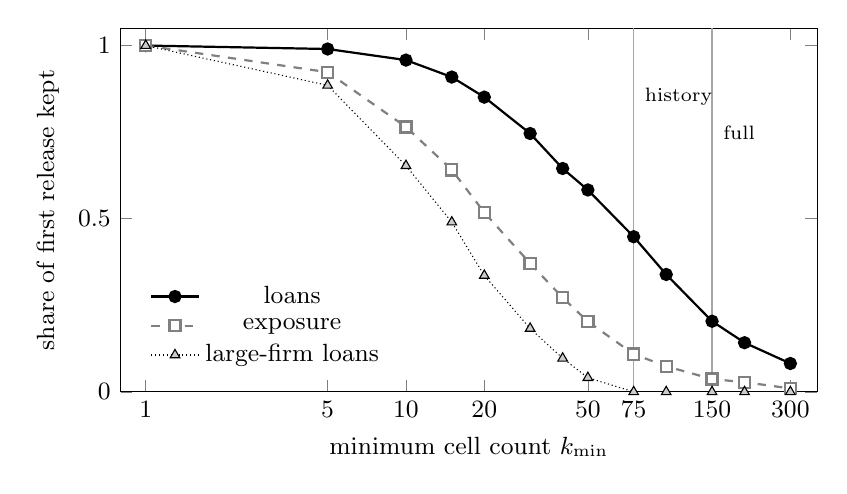
\begin{tikzpicture}
\begin{axis}[width=0.86\textwidth,height=6.2cm,xmode=log,log basis x=10,
  xmin=0.8,xmax=380,ymin=0,ymax=1.05,
  xtick={1,5,10,20,50,75,150,300},xticklabels={1,5,10,20,50,75,150,300},
  xlabel={minimum cell count $k_{\min}$},ylabel={share of first release kept},
  legend style={at={(0.03,0.04)},anchor=south west,font=\small,draw=none,fill=none},
  tick label style={font=\small},label style={font=\small}]
\addplot[black,thick,mark=*,mark options={fill=black}] coordinates {
 (1,1.000)(5,0.990)(10,0.958)(15,0.909)(20,0.851)(30,0.746)(40,0.645)(50,0.583)
 (75,0.448)(100,0.339)(150,0.204)(200,0.142)(300,0.082)};
\addlegendentry{loans}
\addplot[gray,thick,dashed,mark=square*,mark options={fill=white,solid}] coordinates {
 (1,1.000)(5,0.923)(10,0.765)(15,0.641)(20,0.518)(30,0.371)(40,0.272)(50,0.203)
 (75,0.109)(100,0.074)(150,0.037)(200,0.028)(300,0.010)};
\addlegendentry{exposure}
\addplot[black,densely dotted,mark=triangle*,mark options={fill=gray!40,solid}] coordinates {
 (1,1.000)(5,0.885)(10,0.653)(15,0.490)(20,0.336)(30,0.183)(40,0.097)(50,0.041)
 (75,0.000)(100,0.000)(150,0.000)(200,0.000)(300,0.000)};
\addlegendentry{large-firm loans}
\draw[gray!70] (axis cs:75,0) -- (axis cs:75,1.05);
\draw[gray!70] (axis cs:150,0) -- (axis cs:150,1.05);
\node[font=\scriptsize,anchor=south west] at (axis cs:76,0.80) {history};
\node[font=\scriptsize,anchor=south west] at (axis cs:152,0.70) {full};
\end{axis}
\end{tikzpicture}
% source: artifacts-robustness/robustness.json (coverage)
\caption{What each floor keeps of the first release on the synthetic register: loans
(solid, filled circles), exposure (dashed, open squares) and loans to large firms
(dotted, triangles). Vertical lines mark the floors for the pooled adversary with the
history (75) and with a reading per vintage as well (150).}
\label{c13:fig-keeps}
\end{figure}

The gap between the curves has a simple source, which Proposition~\ref{c13:prop-keep}
states. A floor removes whole cells, the cells with the fewest loans; if those cells
hold the larger loans, the exposure share kept must fall below the loan share kept.

\begin{proposition}[Suppression costs exposure faster than loans]\label{c13:prop-keep}
Let cell $c$ of a release hold $n_c$ loans with mean exposure $m_c$, and let a floor
keep the set $S$ of cells with $n_c \ge k$. Write $L_S = \sum_{c\in S} n_c / \sum_c n_c$
for the share of loans kept, $E_S$ for the share of exposure kept, and $\mu_S$ and
$\mu$ for the mean exposure per loan in $S$ and in the whole release. Then
\begin{equation}\label{c13:eq-keep}
E_S = L_S \, \frac{\mu_S}{\mu}.
\end{equation}
If every removed cell has a mean exposure at least as large as every kept cell, then
$E_S \le L_S$, with equality only if $\mu_S = \mu$.
\end{proposition}

The identity holds for any floor on any file. On the register, at the floor of 150,
$E_S/L_S = 0.037/0.204 = 0.18$, so the loans that survive the floor carry on average
less than a fifth of the mean exposure of the first release.
% source: arithmetic on artifacts-robustness/robustness.json (coverage at 150: exposure_share 0.0373, loan_share 0.2044)
The condition of the second part is sufficient and not necessary, and on this
register it holds approximately: large firms are 3 per cent of borrowers, their log
mean exposure is two log units above the next class, and their few loans sit in the
thinnest cells. The misconception the chapter opened with assumes $\mu_S = \mu$, which
is the one case in which counting records measures the loss.

A file that meets the tolerance against a history-aware adversary is therefore not
the file its users asked for. It has lost the borrowers that concentration and
supervisory analysis are about, and most of the borrowers with several lenders, who
fall from 6{,}942 at no suppression to 2{,}747 at 75 and 1{,}194 at 150.
% source: artifacts-robustness/robustness.json (coverage: multi_lender_borrowers_kept)
The utility measure of Table~\ref{c13:tab-harms} makes the same point from the side of
the analyses: at $k_{\min}=20$ the weighted loss is 0.254, almost all of it from
sectoral exposure and lender-level supervision, at 0.531 and 0.435, while
concentration and the arrears ratio lose 0.015 and 0.016.
% source: paper/bis_ifc_full.tex l.1999-2003
Against such an adversary a loan-level release is the wrong product. Aggregates with a
contributor rule, or access to the loan-level file in a secure setting under the Five
Safes \citep{desai2016}, where the declared adversary no longer holds the file, are the
realistic options.

\paragraph{Size-class floors.} The subgroup control asks more. When every size class
must meet the tolerance, with the largest firms audited on their own stratified draw
of 4{,}000 targets, the per-release floor is 20, pooling with the history needs 200,
and for the full pooled attack no level up to 200 passes (last column of
Table~\ref{c13:tab-floors}). From $k_{\min}=75$ no large-firm loan is released, so
that class has no target to protect and the subgroup floors above 75 are set by the
other classes. These floors were selected by the same fixed-sequence rule and not
confirmed on a second draw. Under the subgroup control the per-release answer is
therefore 20 and not 1.
% source: paper/bis_ifc_full.tex l.2287-2296; paper/generated/table_robustness.tex

Tomás reads the figure when Naledi sends it to him. His study is about large firms,
and the curve for large-firm loans reaches zero at the floor his file would need. He
asks whether he could work on the full file in the Bank's secure room instead. That
is the answer Naledi had expected to give him, and it is now in the record with its
reason.

\section{How far the floors move}\label{c13:sec-sensitivity}

Every floor so far rests on one tolerance, one register draw and one value of the
adversary's reading precision. Each of the three can move it.

\paragraph{The tolerance.} Table~\ref{c13:tab-tol} repeats the selection at four
tolerances from the same draw, before confirmation, which is why pooling with the
history shows 50 at a tolerance of 0.12 where Table~\ref{c13:tab-floors} shows the
confirmed 75. At 0.05 the per-release floor is 40, pooling with the history needs 300,
and the full attack has no floor up to 300; at 0.20 the three floors are 1, 5 and 30.
The insider has no floor at any of them. A committee unsure of its tolerance should
read the whole table, since the floor moves by an order of magnitude across this
range, and Chapter~\ref{ch:tolerance} sets out how a stated harm weight implies a
tolerance.
% source: paper/generated/table_tolerance_floors.tex

\begin{table}[ht]
\centering
\caption{Floor selected at four tolerances on the selection draw, before
confirmation. ``None'' means no level up to 300 passes.}
\label{c13:tab-tol}
\small
\begin{tabular}{lrrrr}
\toprule
Tolerance & One release & Pooling, history & Full pooled & Insider \\
\midrule
0.05 & 40 & 300 & none & none \\
0.09 & 5  & 100 & 200  & none \\
0.12 & 1  & 50  & 150  & none \\
0.20 & 1  & 5   & 30   & none \\
\bottomrule
\end{tabular}
% source: paper/generated/table_tolerance_floors.tex
\end{table}

\paragraph{The register draw and the reading precision.} Table~\ref{c13:tab-rep}
repeats the choice over 20 independent register draws and three values of the
standard deviation of the adversary's log-exposure reading, with 2{,}000 targets per
level. At 0.6, the value used so far, the per-release floor is 1 in every draw,
pooling with the history gives a median of 75 with a range of 40 to 75, and the full
attack a median of 150 with a range of 100 to 150. With a reading twice as precise,
at 0.3, the medians are 20, 150 and 300, and for the full attack no level up to 300
passes in 3 of the 20 draws. At 1.0 they are 1, 40 and 75.
% source: paper/generated/table_replication.tex

\begin{table}[ht]
\centering
\caption{Floors over 20 independent register draws, 2{,}000 targets per level, by the
standard deviation of the adversary's log-exposure reading. Median floor with the
smallest and largest in brackets; the superscript counts draws in which no level up
to 300 passed.}
\label{c13:tab-rep}
\small
\begin{tabular}{lrrr}
\toprule
Reading SD & One release & Six vintages, history & Six vintages, history, reading each \\
\midrule
0.3 & 20 [10, 20] & 150 [150, 200] & 300 [300, none]$^{3}$ \\
0.6 & 1 [1, 1]    & 75 [40, 75]    & 150 [100, 150] \\
1.0 & 1 [1, 1]    & 40 [30, 40]    & 75 [50, 100] \\
\bottomrule
\end{tabular}
% source: paper/generated/table_replication.tex
\end{table}

The reading precision moves the floor more than anything else varied, and it is the
input an institution most needs to argue for. At fixed precision the floor stays in a
narrow band across register draws. For the full attack at $k_{\min}=150$ the rate has a
between-register standard deviation of 0.0073 over the 20 draws, with a chi-square
interval on 19 degrees of freedom from 0.006 to 0.011. The binomial standard error of
one draw of 2{,}000 targets at the mean rate is 0.0064, inside that interval, so the
register draw may add nothing or may add a design standard deviation of up to about
0.009. Twenty draws do not estimate the design term well.
% source: paper/bis_ifc_full.tex l.2373-2383
Chapter~\ref{ch:estimate} treats this split of variance between the simulation and
the design.

\paragraph{A chain of audits.} The same choice can be run as one release chain, a
fixed sequence of tests from the strictest floor down with all three outside attacks
declared at once (Chapter~\ref{ch:monitoring}). Over 20 independent target streams it
chose 150 in 19 and 100 once, against an estimated true floor of 100, and no stream
chose an unsafe floor. The gap to 100 comes from the full attack's risk at that floor,
0.116, which lies so close to the tolerance that the audit's capped bet certifies it
only by chance.
% source: paper/bis_ifc_full.tex l.2313-2320; artifacts-neural/neural_pipeline.json (plug_in floors: 150 in 19 streams, 100 in 1)

\paragraph{Rotating the pseudonym.} The pooled attacks match loans across vintages
through a pseudonym that persists. Chapter~\ref{ch:programmes} discussed rotation as a
remedy; the register measures it. With exposure published exactly, the pair of key
and exposure is unique for every first-release loan at every floor tested, a share of
1.000, so the published fields alone relink every loan and rotation gives no
protection. With exposure rounded to one significant figure the pair relinks 0.104 of
loans at $k_{\min}=1$, falling to 0.057 at 20 and 0.010 at 150.
% source: artifacts-robustness/robustness.json (relink_share, relink_share_rounded_1_digit)
Rotation together with rounding would then remove most of the linkage that the
persistent pseudonym gives. These shares count loans that could be joined; the attacks
were not rerun with rotation, so they bound linkability and are not risk figures.

\paragraph{What the attack needs.} Table~\ref{c13:tab-ablation} withdraws the
adversary's auxiliary information one field at a time under $k$-anonymity at $k=5$,
then keeps all four fields and misstates the dispersion of the exposure reading in
the adversary's own likelihood.

\begin{table}[ht]
\centering
\caption{What the attack needs, and an adversary with a wrong model, under
$k$-anonymity at $k=5$. Calibration error is the gap between the average posterior
the adversary reports and the share of its guesses that are right.}
\label{c13:tab-ablation}
\small
\begin{tabular}{lrrrr}
\toprule
Adversary holds & Fields & Risk & Precision & Calibration error \\
\midrule
All four fields             & 4 & 0.081 & 0.672 & 0.000 \\
No exposure reading         & 3 & 0.025 & --    & 0.002 \\
No size class               & 3 & 0.042 & 0.500 & 0.002 \\
Region and exposure only    & 2 & 0.004 & --    & 0.001 \\
\midrule
Assumed $\sigma \times 0.5$ & 4 & 0.079 & 0.384 & 0.073 \\
Assumed $\sigma \times 1$   & 4 & 0.079 & 0.667 & 0.003 \\
Assumed $\sigma \times 2$   & 4 & 0.079 & 1.000 & 0.039 \\
\bottomrule
\end{tabular}
% source: paper/generated/table_ablation.tex
\end{table}

Without the exposure reading the adversary reaches 0.025 and never passes the
decision threshold, because a released cell has at least five members and nothing
separates them. Holding only region and the reading it reaches 0.004. The key narrows
the candidates to a cell and the reading separates the members of that cell, and
neither does much alone. When the adversary misstates its own dispersion, its success
stays at 0.079 whether it halves or doubles the true value, because the
highest-scoring candidate does not change when the same density is rescaled over the
same candidates. What moves is
calibration, from 0.003 to as much as 0.073.
% source: paper/generated/table_ablation.tex
An overconfident attacker still identifies the same records. An institution that
estimates risk under a misspecified adversary model reports a number whose stated
confidence is wrong, and the falsification tests of Chapter~\ref{ch:falsification}
are the check that catches it.

Grace reads the decision record some months later. She finds the selection at 50,
the failed confirmation at 50, the confirmed 75, and the note that 150 is required if
the adversary also tracks the loan's exposure month by month. What she checks is
whether the record says which adversary the Bank declared and why. It does: the
outside researcher without the history, for the secure-room file, and the full
pooled adversary for anything published.

\section{Arguing the adversary's reading precision}\label{c13:sec-precision}

The floors depend on how well the adversary reads the attribute it uses, and that precision cannot be estimated from the synthetic register. It has to be argued, and the argument has five steps. First, list the sources an outsider could hold for the key attributes: public records, a commercial file, an earlier release, a colleague's knowledge. Second, for each source, state its error rate or noise and the evidence for it. Third, state how an adversary would combine sources and whether combining lowers the error. Fourth, run the floors across the plausible range of precision and not at one value, and report the range, in the form of Table~\ref{c13:tab-rep}. Fifth, sign the scenario with the range and the reason for its upper end. A floor that is stable across the range can be carried into a signed threshold. A floor that moves a lot is reported with its range.

\section{What the evaluation does not settle}\label{c13:sec-limits}

The register is synthetic, and every result in this chapter holds on the synthetic
register only. Its parameters are chosen, and two of the generator's simplifications
bear on the floors. Exposure is constant across vintages, so without the history the
other vintages carry no information; with amortising balances they would. And whether
a loan is live is independent of its key and exposure. The credit module would take a
real register in place of the simulated one, but it has not been run on one.

The adversary is one adversary, strong in some respects and weak in others. It holds
the key exactly, uses a persistent pseudonym, knows the true error model of its
reading and, in the pooled attacks with history, the loan's live vintages. It does not
use arrears status, lender identity or a longer history. The evaluation is therefore
neither a lower nor an upper bound on what an adversary can achieve. Its value is
comparative, since every policy faces the same attacker, and conditional, since every
floor holds for the adversary declared.

Finally, the policies are compared as they are usually configured. A contributor rule
calibrated on the pooled programme would do better than the row for it in
Table~\ref{c13:tab-eval}: the same lever, calibrated on the programme, changes the
outcome.

\section{The answer}

The floor depends on what the declared adversary knows. At a tolerance of 0.12 on
this register it is 1 against an adversary with one release or without the loan's
history, 75 against one who knows the history, 150 against one who also tracks the
exposure in every vintage, and no floor at all against an insider who reads exposure
precisely. Protecting every size class moves the per-release floor from 1 to 20 and
the pooled floors to 200 or beyond. What is left of the file falls much faster than
the count of loans: at 75 the file keeps 45 per cent of loans and 11 per cent of
exposure, at 150 it keeps 20 per cent and 4 per cent, and from 75 up it keeps no loan
to a large firm. Suppression removes thin cells, and in a credit register the thin
cells carry the money, so the cost of a floor has to be stated in exposure and in the
analyses lost. Against a history-aware adversary the loan-level file is the wrong
product, and the institution should offer aggregates with a contributor rule or
access in a secure setting.

\begin{inpractice}[In practice: a loan-level credit file]
Declare the adversaries before choosing a floor, and for each say whether it knows
the loan's history and how precisely it reads exposure, since these two inputs move
the floor more than anything else. Choose the floor by fixed-sequence testing on the
exact upper bound and confirm it on a fresh draw. Report the cost of the floor in
exposure, in loans to each size class and in the analyses the register serves, not
in records alone. Assess the other four harms with their own levers: an attribute
rule for status, a predictive-value tolerance for alleged relationships, a contributor
or dominance rule for aggregates, and a count rule for differencing. If the floor a
declared adversary requires removes the borrowers the users need, offer a secure
setting or aggregates in place of the file. Rotating a keyed pseudonym helps only when
the published fields cannot relink loans on their own, so test the relink share first.

\sloppy\smallskip\noindent\textit{In the software.} The register and the five harms are in
\texttt{privacy\_risk.credit} (\texttt{make\_credit\_register},
\texttt{borrower\_identification}, \texttt{relationship\_disclosure},
\texttt{status\_inference}, \texttt{reconstruction\_from\_totals},
\texttt{differencing\_risk}). The policies and attacks are in
\texttt{privacy\_risk.evaluation} (\texttt{identification\_attack},
\texttt{programme\_attack}, \texttt{relink\_share}), and
\texttt{scripts/programme\_robustness.py} produces the floors, the tolerance table, the
replication and the relink shares. The relink share is short enough to show whole:
\begin{lstlisting}
def relink_share(register, policy, exposure_digits=None):
    key = register.key()
    first = released_rows(register, policy, 0)
    published = round_significant(register.exposure[first], exposure_digits)
    pairs = np.stack([key[first], np.log(published)], axis=1)
    _, inverse, counts = np.unique(pairs, axis=0, return_inverse=True,
                                   return_counts=True)
    return float(np.mean(counts[inverse.ravel()] == 1))
\end{lstlisting}
\end{inpractice}

\section{Proofs}

\begin{proof}[Proof of Proposition~\ref{c13:prop-diff}]
Since $A$ and $D$ are independent Poisson variables with mean $\lambda$,
$\Prob(A=a, D=d) = e^{-2\lambda}\lambda^{a+d}/(a!\,d!)$. The event $|A-D|=1$ is the
disjoint union of $\{A = d+1, D = d\}$ and $\{A = d, D = d+1\}$ over $d \ge 0$, and the
two families have equal probability by symmetry, so
\[
\Prob(|A-D|=1) = 2e^{-2\lambda}\sum_{d=0}^{\infty}\frac{\lambda^{2d+1}}{d!\,(d+1)!}.
\]
The event $A+D=1$ within it is the case $d=0$ of both families, with probability
$2e^{-2\lambda}\lambda$. Dividing gives
\[
\Prob\bigl(A+D=1 \bigm| |A-D|=1\bigr)
= \frac{\lambda}{\sum_{d\ge 0}\lambda^{2d+1}/(d!\,(d+1)!)}
= \Bigl(\sum_{d=0}^{\infty}\frac{\lambda^{2d}}{d!\,(d+1)!}\Bigr)^{-1}.
\]
The series $\sum_{d\ge 0}(\lambda)^{2d+1}/(d!\,(d+1)!)$ is the power series of
$I_1(2\lambda)$, which gives the second form. Each term $\lambda^{2d}/(d!\,(d+1)!)$
with $d \ge 1$ is strictly increasing in $\lambda > 0$ and the $d=0$ term equals one,
so the sum is strictly increasing and its reciprocal strictly decreasing, and the sum
tends to one as $\lambda \to 0$.
\end{proof}

\begin{proof}[Proof of Proposition~\ref{c13:prop-insider}]
The Gaussian log likelihood of candidate $j$ is $-(y-x_j)^2/(2\sigma^2)$ up to a
constant, so the attack names a candidate nearest to $y$. For part 1, suppose
$|e| < g/2$. Then $|y - x_t| = |e| < g/2$, and for every $j \ne t$,
$|y - x_j| \ge |x_j - x_t| - |e| > g - g/2 = g/2$. The target is then the unique
nearest candidate and is named. Hence the probability of success is at least
$\Prob(|e| < g/2) = 2\Phi(g/(2\sigma)) - 1$, which does not involve $n$ and tends to
one as $\sigma \to 0$ for fixed $g > 0$. For part 2, the $r$ candidates that publish
the target's value have the same likelihood for every $y$. Whenever the target is
among the maximisers, so are the other $r-1$, and a uniform choice among at least $r$
maximisers names the target with probability at most $1/r$. Whenever the target is
not among the maximisers, the attack fails. Averaging over $e$ gives the bound.
\end{proof}

\begin{proof}[Proof of Proposition~\ref{c13:prop-keep}]
Let $N = \sum_c n_c$ and $N_S = \sum_{c \in S} n_c$. The total exposure is
$\sum_c n_c m_c = N\mu$ and the exposure kept is $\sum_{c\in S} n_c m_c = N_S \mu_S$, so
$E_S = N_S\mu_S/(N\mu) = L_S\,\mu_S/\mu$, which is \eqref{c13:eq-keep}. For the
inequality, let $\bar S$ be the removed cells and $\mu_{\bar S}$ their mean exposure
per loan, defined when $\bar S$ holds a loan; if it holds none, $L_S = E_S = 1$. Under
the condition, every $m_c$ with $c \in S$ is at most every $m_{c'}$ with
$c' \in \bar S$, so the loan-weighted mean over $S$ is at most that over $\bar S$:
$\mu_S \le \mu_{\bar S}$. Since $\mu = L_S\mu_S + (1-L_S)\mu_{\bar S}$ is a convex
combination of the two, $\mu_S \le \mu$, and \eqref{c13:eq-keep} gives
$E_S \le L_S$. Equality requires $\mu_S = \mu$.
\end{proof}
